%% This file contains example tex and sweave, e.g., for inserting figures, referencing figures, intext code.


\documentclass[10pt,a4paper]{book}\usepackage[]{graphicx}\usepackage[]{color}
%% maxwidth is the original width if it is less than linewidth
%% otherwise use linewidth (to make sure the graphics do not exceed the margin)
\makeatletter
\def\maxwidth{ %
  \ifdim\Gin@nat@width>\linewidth
    \linewidth
  \else
    \Gin@nat@width
  \fi
}
\makeatother

\definecolor{fgcolor}{rgb}{0.345, 0.345, 0.345}
\newcommand{\hlnum}[1]{\textcolor[rgb]{0.686,0.059,0.569}{#1}}%
\newcommand{\hlstr}[1]{\textcolor[rgb]{0.192,0.494,0.8}{#1}}%
\newcommand{\hlcom}[1]{\textcolor[rgb]{0.678,0.584,0.686}{\textit{#1}}}%
\newcommand{\hlopt}[1]{\textcolor[rgb]{0,0,0}{#1}}%
\newcommand{\hlstd}[1]{\textcolor[rgb]{0.345,0.345,0.345}{#1}}%
\newcommand{\hlkwa}[1]{\textcolor[rgb]{0.161,0.373,0.58}{\textbf{#1}}}%
\newcommand{\hlkwb}[1]{\textcolor[rgb]{0.69,0.353,0.396}{#1}}%
\newcommand{\hlkwc}[1]{\textcolor[rgb]{0.333,0.667,0.333}{#1}}%
\newcommand{\hlkwd}[1]{\textcolor[rgb]{0.737,0.353,0.396}{\textbf{#1}}}%

\usepackage{framed}
\makeatletter
\newenvironment{kframe}{%
 \def\at@end@of@kframe{}%
 \ifinner\ifhmode%
  \def\at@end@of@kframe{\end{minipage}}%
  \begin{minipage}{\columnwidth}%
 \fi\fi%
 \def\FrameCommand##1{\hskip\@totalleftmargin \hskip-\fboxsep
 \colorbox{shadecolor}{##1}\hskip-\fboxsep
     % There is no \\@totalrightmargin, so:
     \hskip-\linewidth \hskip-\@totalleftmargin \hskip\columnwidth}%
 \MakeFramed {\advance\hsize-\width
   \@totalleftmargin\z@ \linewidth\hsize
   \@setminipage}}%
 {\par\unskip\endMakeFramed%
 \at@end@of@kframe}
\makeatother

\definecolor{shadecolor}{rgb}{.97, .97, .97}
\definecolor{messagecolor}{rgb}{0, 0, 0}
\definecolor{warningcolor}{rgb}{1, 0, 1}
\definecolor{errorcolor}{rgb}{1, 0, 0}
\newenvironment{knitrout}{}{} % an empty environment to be redefined in TeX

\usepackage{alltt}
\usepackage{url}
\usepackage{fancybox}
\usepackage{textcomp}
\usepackage{float}
\usepackage[T1]{fontenc}
\usepackage{mdframed}
\newcommand{\midtilde}{\raisebox{0.5ex}{\texttildelow}}

%% Next chunk is setup for simple boxes
%% Needs to go at the start of any chapter with boxes
\mdfdefinestyle{theoremstyle}{%
  linecolor=blue,linewidth=2pt,%
  frametitlerule=true,%
  innertopmargin=\topskip,
}
\mdtheorem[style=theoremstyle]{text_box}{Box}[chapter]
\IfFileExists{upquote.sty}{\usepackage{upquote}}{}
\begin{document}
%% \SweaveOpts{concordance=TRUE}

\chapter{A guide for writing chapters}

\section{A section title}

\subsection{A subsection title}

\subsubsection{A sub-subsection title}

\subsubsection{How to compile a chapter}

In Rstudio preferences, Sweave, set "Weave Rnw files using" \textbf{knitr}. When ready, click "Compile PDF" button.

\subsection{Inline code, url, emphasis, etc.}

If we want some inline code that isn't evaluated do it like this: you can use the \texttt{plot()} function to plot graphs. Don't forget to put a slash before underscores, e.g. \texttt{group\_by}. Evaluated code goes like this: Pi = 3.1415927.

A URL: \url{www.r4all.org}.

How to \emph{emphasise some text} by making it italic. Or by making it \textbf{bold}.


\subsection{Work-along-icons in the margins}

\marginpar{work-a-long icon here}




\subsection{Code chunks}

Do it like this:

\begin{knitrout}
\definecolor{shadecolor}{rgb}{0.969, 0.969, 0.969}\color{fgcolor}\begin{kframe}
\begin{alltt}
\hlstd{x} \hlkwb{<-} \hlnum{1}\hlopt{:}\hlnum{10}
\end{alltt}
\end{kframe}
\end{knitrout}

Chunk options here: \url{http://yihui.name/knitr/options/}

Including code tidying:
\begin{knitrout}
\definecolor{shadecolor}{rgb}{0.969, 0.969, 0.969}\color{fgcolor}\begin{kframe}
\begin{alltt}
\hlstd{lady.matrix} \hlkwb{<-} \hlkwd{tapply}\hlstd{(lady}\hlopt{$}\hlstd{number,} \hlkwd{list}\hlstd{(}\hlkwc{colour} \hlstd{= lady}\hlopt{$}\hlstd{colour,}
    \hlkwc{Habitat} \hlstd{= lady}\hlopt{$}\hlstd{Habitat), sum)}
\end{alltt}
\end{kframe}
\end{knitrout}

See the difference:
\begin{knitrout}
\definecolor{shadecolor}{rgb}{0.969, 0.969, 0.969}\color{fgcolor}\begin{kframe}
\begin{alltt}
\hlstd{lady.matrix} \hlkwb{<-} \hlkwd{tapply}\hlstd{(lady}\hlopt{$}\hlstd{number,} \hlkwd{list}\hlstd{(}\hlkwc{colour}\hlstd{=lady}\hlopt{$}\hlstd{colour,} \hlkwc{Habitat}\hlstd{=lady}\hlopt{$}\hlstd{Habitat), sum)}
\end{alltt}
\end{kframe}
\end{knitrout}

\subsection{Importing data}

Load the data from github with something like this:



Note that we use the chunk options \texttt{echo=FALSE} and \texttt{message=FALSE} because we don't want this code to appear in the chapter. Rather, we want this to appear:

\begin{knitrout}
\definecolor{shadecolor}{rgb}{0.969, 0.969, 0.969}\color{fgcolor}\begin{kframe}
\begin{alltt}
\hlstd{lady} \hlkwb{<-} \hlkwd{read.csv}\hlstd{(}\hlstr{"ladybirds.csv"}\hlstd{)}
\end{alltt}
\end{kframe}
\end{knitrout}

Though we don't want this run, so use the chunk option \texttt{eval=FALSE}.

\subsubsection{Figures}

Use a separate code chunk for each figure. The first chunk option is the figure label, to be used when making and in text citation (cross reference) to the figure (e.g., Fig. \ref{fig:x_y_squared}).

\begin{knitrout}
\definecolor{shadecolor}{rgb}{0.969, 0.969, 0.969}\color{fgcolor}\begin{kframe}
\begin{alltt}
\hlstd{x} \hlkwb{<-} \hlkwd{seq}\hlstd{(}\hlopt{-}\hlnum{10}\hlstd{,} \hlnum{10}\hlstd{,} \hlnum{0.1}\hlstd{)}
\hlkwd{plot}\hlstd{(x, x}\hlopt{^}\hlnum{2}\hlstd{,} \hlkwc{type}\hlstd{=}\hlstr{"l"}\hlstd{)}
\end{alltt}
\end{kframe}\begin{figure}[H]

{\centering 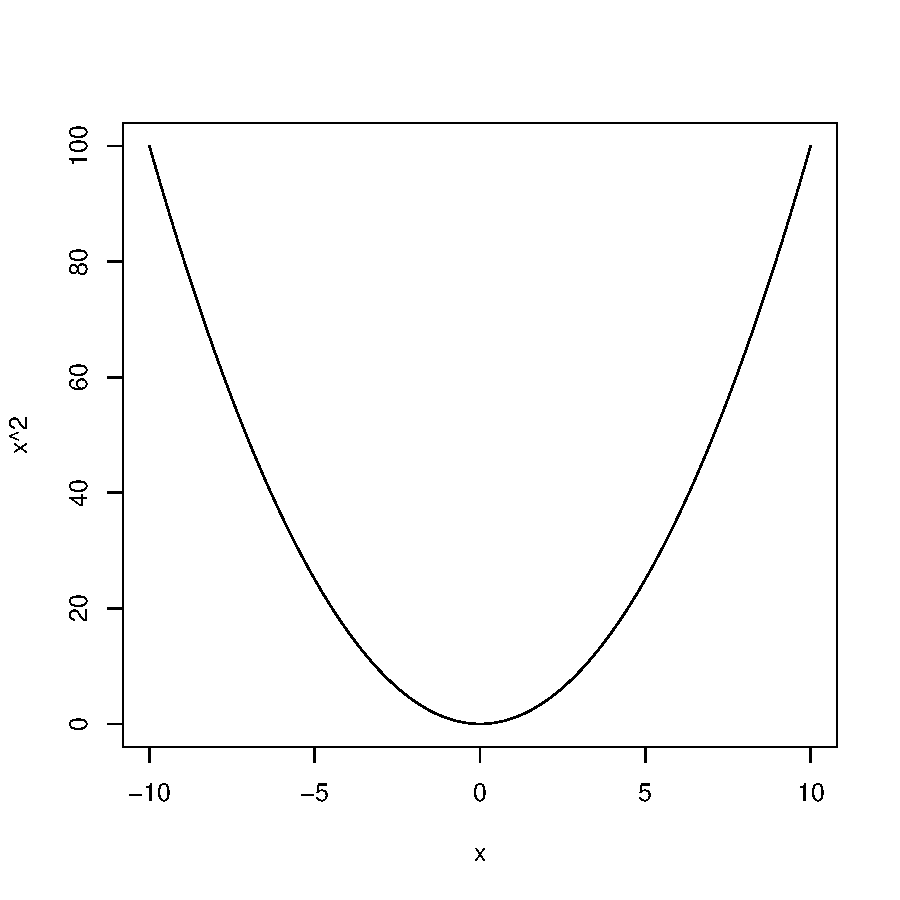
\includegraphics[width=0.7\textwidth]{figure/x_y_squared-1} 

}

\caption[A graph of y = x squared]{A graph of y = x squared}\label{fig:x_y_squared}
\end{figure}


\end{knitrout}


\subsubsection{Images}

Save the image as a pdf, put it in the images folder of the chapter folder, and insert it. Reference it as usual, e.g., Fig. \ref{fig:Andrew_Heath}.


\begin{figure}[]
\centering
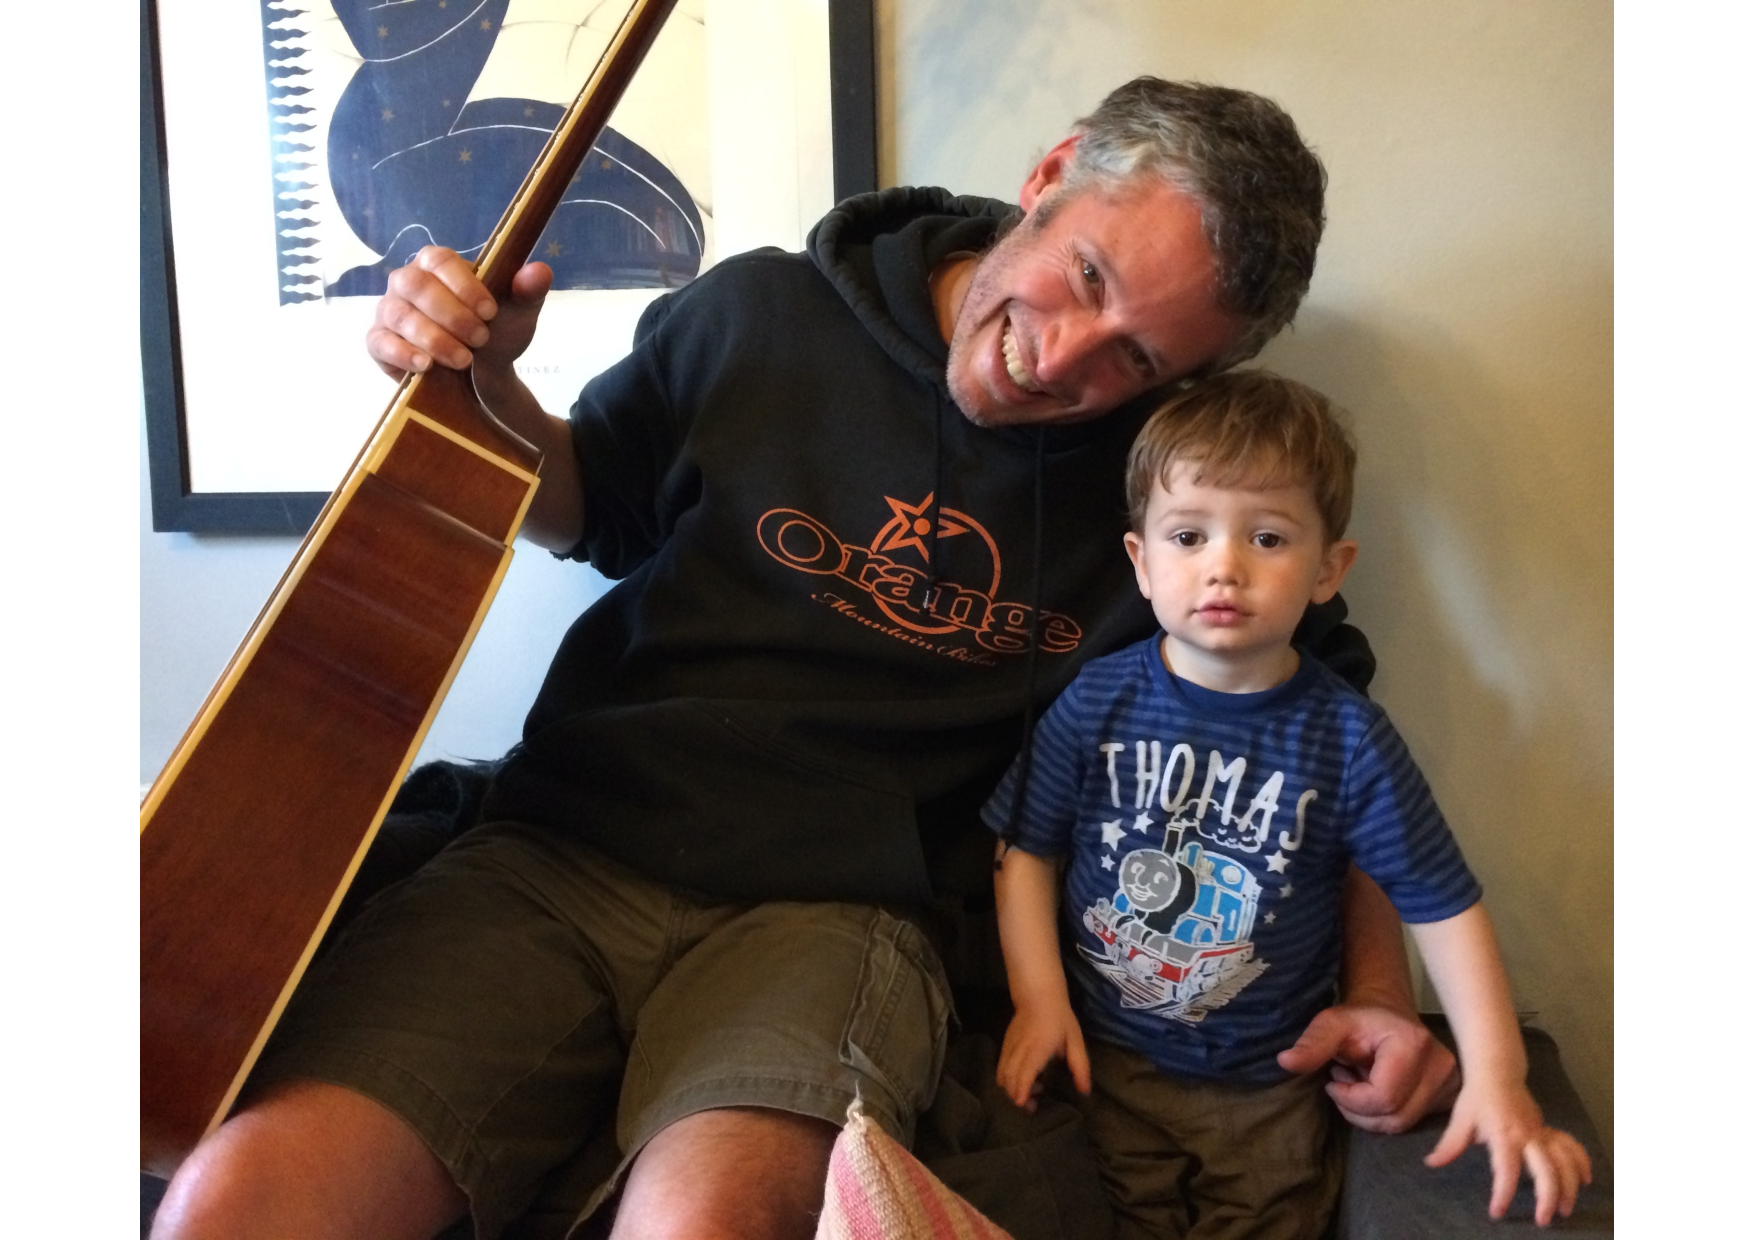
\includegraphics[width=200pt]{images/IMG_1199.pdf}
\caption{Andrew and Heath hanging out!}
\label{fig:Andrew_Heath}
\end{figure}


\newpage

\subsubsection{Boxes}

Keep them simple; i.e., leave for OUP to typeset. So do like this, probably grouped at end of chapters (e.g., Box \ref{Box_test}).



\begin{text_box}[The chi-square contingency table analysis]

\begin{knitrout}
\definecolor{shadecolor}{rgb}{0.969, 0.969, 0.969}\color{fgcolor}\begin{kframe}
\begin{alltt}
\hlcom{# Clear R's brain}
\hlkwd{rm}\hlstd{(}\hlkwc{list} \hlstd{=} \hlkwd{ls}\hlstd{())}
\hlcom{# Chi-square test Enter the data, as a matrix, with}
\hlcom{# informative dimension names}
\hlstd{lady} \hlkwb{<-} \hlkwd{read.csv}\hlstd{(}\hlstr{"ladybirds.csv"}\hlstd{)}
\hlcom{# Get the total counts per colour and habitat}
\hlstd{lady.matrix} \hlkwb{<-} \hlkwd{tapply}\hlstd{(lady}\hlopt{$}\hlstd{number,} \hlkwd{list}\hlstd{(}\hlkwc{colour} \hlstd{= lady}\hlopt{$}\hlstd{colour,}
    \hlkwc{Habitat} \hlstd{= lady}\hlopt{$}\hlstd{Habitat), sum)}
\hlcom{# use barplot to make an informative and helpful}
\hlcom{# figure}
\hlkwd{barplot}\hlstd{(lady.matrix,} \hlkwc{beside} \hlstd{=} \hlnum{TRUE}\hlstd{,} \hlkwc{col} \hlstd{=} \hlkwd{c}\hlstd{(}\hlstr{"Black"}\hlstd{,}
    \hlstr{"Red"}\hlstd{),} \hlkwc{ylim} \hlstd{=} \hlkwd{c}\hlstd{(}\hlnum{0}\hlstd{,} \hlnum{125}\hlstd{),} \hlkwc{legend} \hlstd{=} \hlnum{TRUE}\hlstd{)}
\hlcom{# perform the chi-square test}
\hlkwd{chisq.test}\hlstd{(lady.matrix)}
\hlcom{# assign the test to an object and examine it,}
\hlcom{# retrieving the expected values}
\hlstd{lady.chi} \hlkwb{<-} \hlkwd{chisq.test}\hlstd{(lady.matrix)}
\hlkwd{names}\hlstd{(lady.chi)}
\hlstd{lady.chi}\hlopt{$}\hlstd{expected}
\end{alltt}
\end{kframe}
\end{knitrout}

If you put a figure, graphic, image, inside a box, don't give it a caption or number:

\vspace{5mm} %5mm vertical space
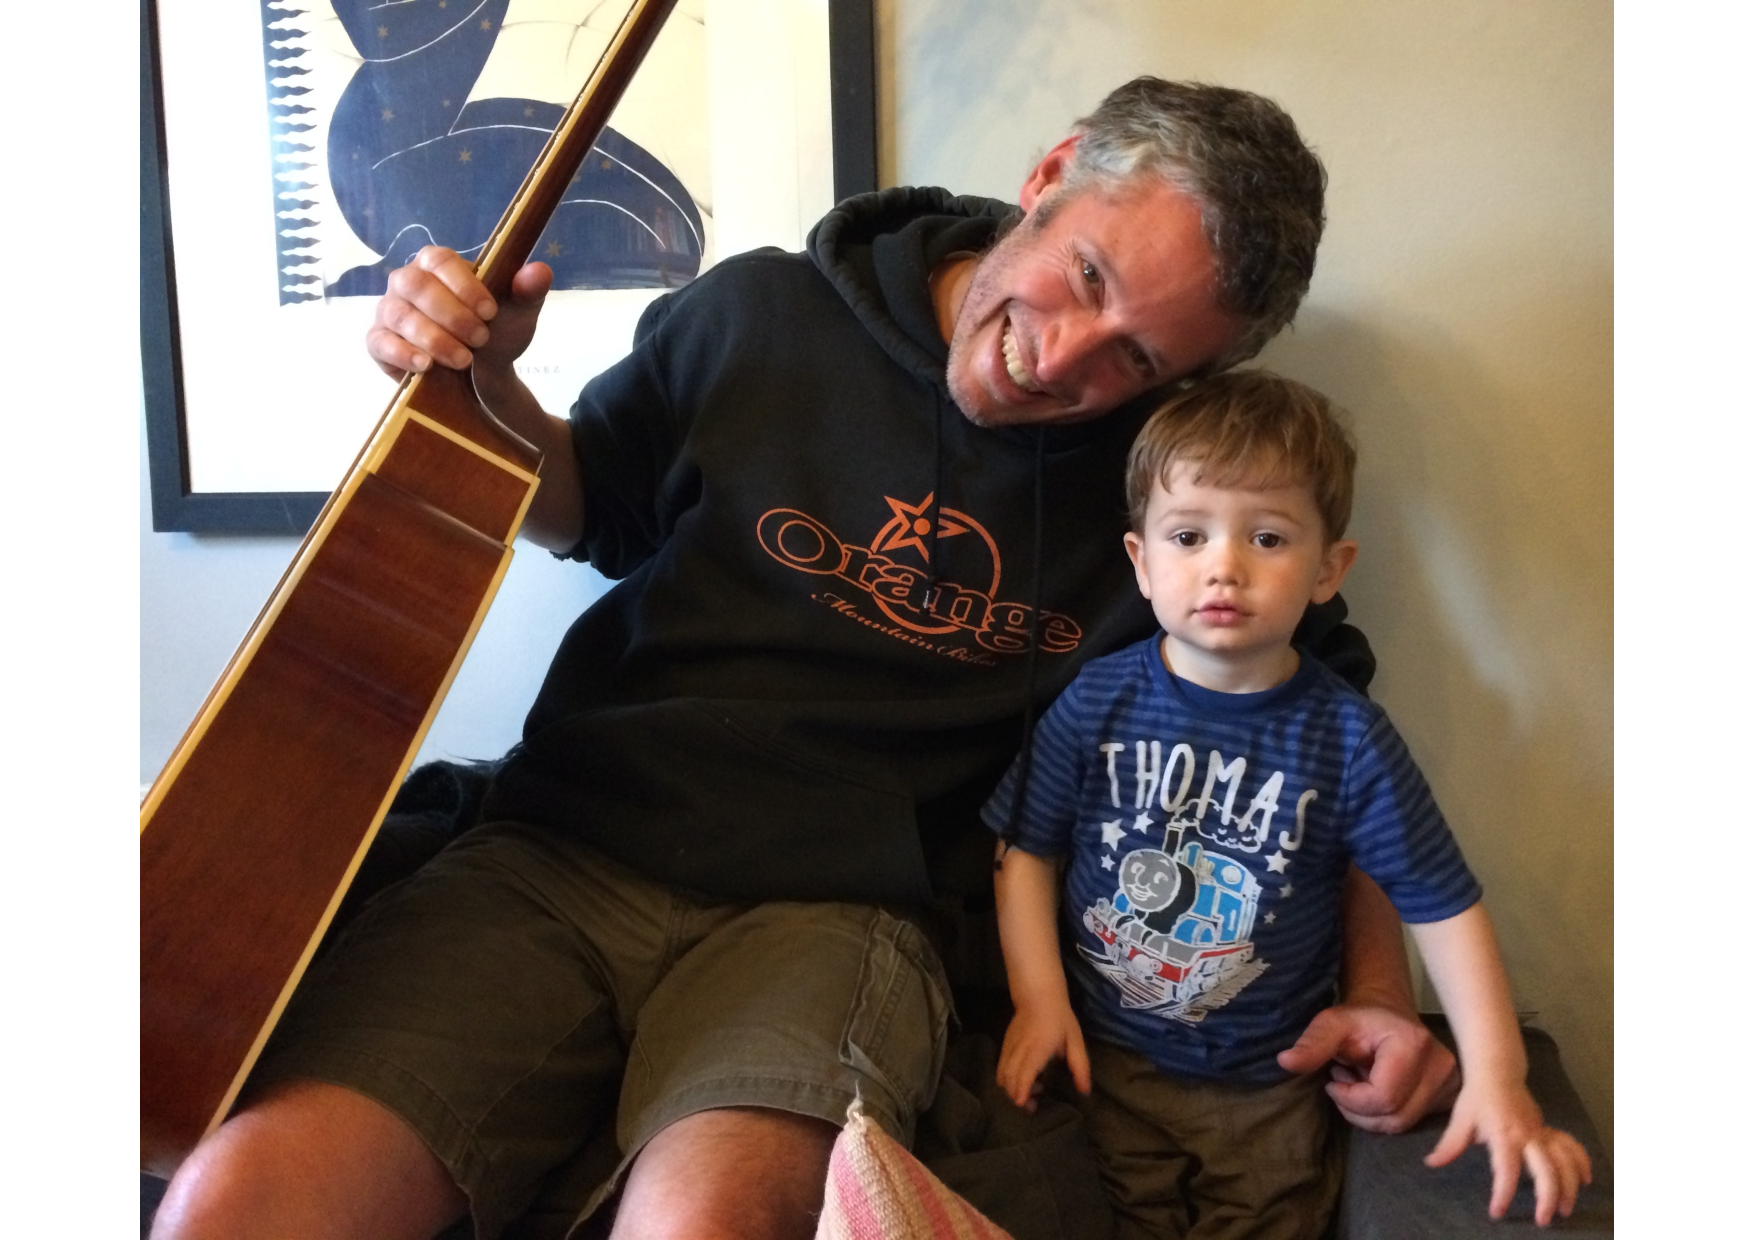
\includegraphics[width=100pt]{images/IMG_1199.pdf}
\vspace{5mm} %5mm vertical space



\label{Box_test}
\end{text_box}



\end{document}
